\documentclass[aspectratio=169]{beamer}


\usepackage[utf8]{inputenc}
\usepackage[spanish]{babel}
\usepackage{amsmath}
\usepackage{amsfonts}
\usepackage{amssymb}
\usepackage{graphicx}
\usepackage{booktabs}
\usepackage{tikz}


\usetheme{Madrid}
\usecolortheme{beaver} 


\title[Simulación Orbital]{Simulación Numérica de Inyección Orbital y \\ cálculo del ángulo de panel solar del satélite}
\subtitle{Propuesta de Proyecto Final - Métodos Numéricos}
\author{} % Campo vacío intencionalmente
\institute{} % Campo vacío intencionalmente
\date{\today}


\begin{document}

% 1. Portada
\begin{frame}
  \titlepage
\end{frame}

% 2. Agenda
\begin{frame}{Agenda}
  \tableofcontents
\end{frame}


\section{Descripción del Proyecto}

\begin{frame}{Evolución del Concepto: De Tierra a Órbita}
  \begin{columns}
    \column{0.55\textwidth}
      \begin{block}{Propuesta Base}
        Seguidor solar estático (Tierra).
      \end{block}
      
      \vspace{0.3cm}
      
      \begin{alertblock}{Nueva Propuesta: Entorno Dinámico}
        Simulación integral de misión aeroespacial:
        \begin{itemize}
            \item \textbf{Fase 1:} Lanzamiento y Ascenso (Física de cohetes).
            \item \textbf{Fase 2:} Inserción en Órbita Terrestre (Mecánica Orbital).
            \item \textbf{Fase 3:} Control de actitud de paneles solares en movimiento.
        \end{itemize}
      \end{alertblock}
    
    \column{0.45\textwidth}
      \centering
      % Primera imagen: Visión general
      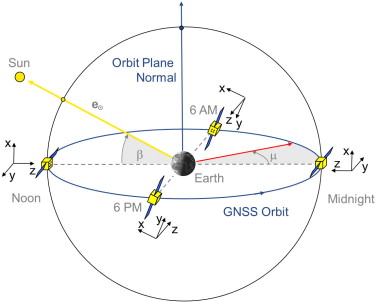
\includegraphics[width=\textwidth]{general_earth_orbit.png}
      \vspace{0.2cm}
      \tiny{\textit{Figura 1: Esquema general de la trayectoria orbital.}}
  \end{columns}
\end{frame}


\section{Objetivos}

\begin{frame}{Objetivo General}
  \begin{center}
    \Large
    Desarrollar un motor de física computacional que integre \textbf{ecuaciones diferenciales ordinarias} y \textbf{métodos de interpolación} para modelar una misión espacial completa.
  \end{center}
\end{frame}

\begin{frame}{Objetivos Específicos}
  \begin{enumerate}
      \item \textbf{Dinámica de Vuelo:} Implementar integración numérica para masa variable y fuerzas no lineales (Arrastre y Gravedad).
      \item \textbf{Atmósfera Numérica:} Modelar la densidad $\rho(h)$ mediante \textbf{interpolación} de datos estándar.
      \item \textbf{Solver Diferencial:} Implementar \textbf{Runge-Kutta 4 (RK4)} "from scratch" comparando precisión vs Euler.
      \item \textbf{Eventos Discretos:} Usar \textbf{búsqueda de raíces} (Newton-Raphson) para detectar eventos (MECO, separación de etapas).
  \end{enumerate}
\end{frame}


\section{Fundamento Matemático}

\begin{frame}{El Modelo Físico: Trayectoria}
  Se resuelve la Segunda Ley de Newton para masa variable en cada paso $\Delta t$:
  
  \begin{equation*}
    \vec{a}(t) = \frac{\vec{T} - \vec{D}(v, \rho) - \vec{g}(h) m(t)}{m(t)}
  \end{equation*}
  
  \vspace{0.5cm}
  Variables Numéricas:
  \begin{itemize}
      \item $\vec{D}$: Arrastre (Interpolación de $\rho$).
      \item $\vec{g}(h)$: Gravedad ($\propto 1/r^2$).
      \item Solver: RK4 para minimizar error global.
  \end{itemize}
\end{frame}

\begin{frame}{Estrategia de Control: Yaw Steering}
  \begin{columns}
    \column{0.6\textwidth}
      Para maximizar la eficiencia energética ($\vec{n} \cdot \vec{s} = 1$), el simulador calculará dos ángulos de control concurrentes:

      \begin{enumerate}
          \item \textbf{Ángulo de Guiñada ($\psi$, Yaw):} Rotación del cuerpo entero del satélite alrededor del eje Nadir (Z) para alinear el eje de los paneles con el plano solar.
          \item \textbf{Ángulo del Panel ($\phi$, Pitch):} Rotación del mecanismo SADM para compensar la elevación.
      \end{enumerate}

      $$ \vec{S}_{panel} = [R_y(\phi)]_{SADM} \cdot [R_z(\psi)]_{Body} \cdot \vec{S}_{inercial} $$

    \column{0.4\textwidth}
      \centering
      % Segunda imagen aquí para ilustrar los vectores y ángulos
      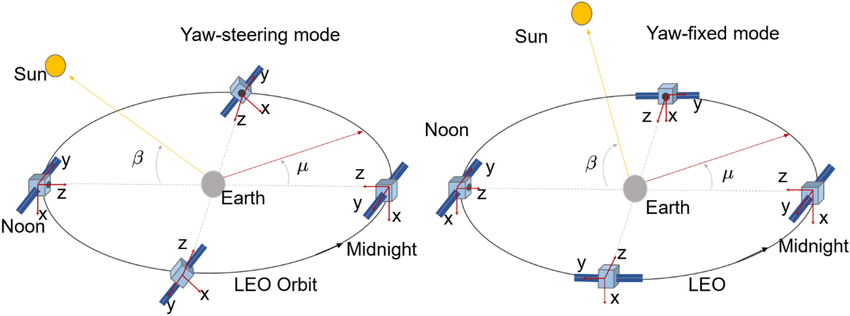
\includegraphics[width=0.9\textwidth]{general_earth_orbit2.png}
      \vspace{0.2cm}
      \tiny{\textit{Figura 2: Geometría vectorial y ángulos de control.}}
  \end{columns}
\end{frame}


\section{Métodos Numéricos}

\begin{frame}{Mapa de Métodos Numéricos}
  \begin{table}[]
    \centering
    \begin{tabular}{@{}lll@{}}
    \toprule
    \textbf{Dominio} & \textbf{Método Numérico} & \textbf{Aplicación} \\ \midrule
    Trayectoria $(x,y)$ & \textbf{Runge-Kutta 4} & Integración de EDOs rígidas. \\
    Atmósfera & \textbf{Interpolación Spline} & Densidad del aire (datos discretos). \\
    Eventos & \textbf{Bisección / Newton} & Tiempos exactos (fin de combustible). \\
    Orientación & \textbf{Álgebra Lineal} & Matrices de Rotación (Yaw/Pitch). \\ \bottomrule
    \end{tabular}
  \end{table} % <--- AQUI ESTABA EL ERROR ANTES
\end{frame}


\section{Tecnología}

\begin{frame}{Arquitectura de Software}
  Enfoque moderno orientado a servicios y reproducibilidad.
  
  \vspace{0.5cm}
  
  \begin{itemize}
      \item \textbf{Core Matemático:} Python + NumPy (Vectorización).
      \item \textbf{Backend/API:} FastAPI (Exposición de datos de telemetría).
      \item \textbf{Despliegue:} Docker \& Docker Compose.
      \item \textbf{Visualización:} Frontend simple con React (JSX/TSX).
  \end{itemize}

  \vspace{0.5cm}
  \centering
  \small{\textit{*El código se ejecuta en contenedores para garantizar independencia del SO. (todo Linux)}}
\end{frame}


\section{Conclusión}

\begin{frame}{Conclusiones y Valor Agregado}
  \begin{itemize}
      \item \textbf{Integralidad:} El proyecto abarca los pilares fundamentales del curso: EDOs (segundo semestre), Raíces e Interpolación.
      \item \textbf{Aplicación Real:} Transición de problemas teóricos a ingeniería aeroespacial simplificada.
      \item \textbf{Implementación:} Desarrollo de algoritmos propios ("from scratch") validando la teoría numérica.
  \end{itemize}
  
  \vspace{1cm}
  \centering
  \textbf{\Large Fin de la presentación}
\end{frame}

\end{document}